%
\documentclass[12pt,letter]{article}

\usepackage[utf8]{inputenc}
\usepackage[usenames,dvipsnames]{xcolor}
\usepackage{color, colortbl}
\usepackage{graphicx}
\usepackage[margin=1in]{geometry}
\usepackage[]{natbib}
\usepackage[]{sidecap}
\usepackage{setspace}
\usepackage{amsmath,amssymb}
\usepackage{defs}
\usepackage{lastpage}
\usepackage{fancyhdr}
\usepackage{pdfpages}
\usepackage{enumitem}
\usepackage{caption}
\usepackage{multicol}

%\usepackage{libertine}
\usepackage{times}
\usepackage[T1]{fontenc}

\setlength{\parindent}{0cm}
\setlength{\parskip}{0.5\baselineskip}
\setlist{nolistsep}

\let\OLDthebibliography\thebibliography
\renewcommand\thebibliography[1]{
  \OLDthebibliography{#1}
  \setlength{\parskip}{0pt}
  \setlength{\itemsep}{0pt plus 0.3ex}
}

\usepackage[pdftex]{hyperref}
\hypersetup {
    bookmarks=true,                    % show bookmarks bar in pdf reader
    pdftitle={NASA Astrophysics Theory Program Proposal},                   
    pdfauthor={Gregory A. Feiden},     % set pdf author
    pdfsubject={Proposal for NASA ROSES 2016 ATP Solicitation}, % pdf subject
    colorlinks=true,                   % false = box link, true = colored links
    linkcolor=black,                   % color of internal links
    citecolor=black,                    % color of citations
    urlcolor=NavyBlue                      % external url color
}
\urlstyle{same}

\captionsetup[table]{labelfont={footnotesize, bf}, textfont={small, sc}, labelsep=newline, labelformat=simple, justification=centering}
\captionsetup[figure]{labelfont={footnotesize, bf}, textfont={small}, labelsep=colon, labelformat=simple}


\citestyle{aa}
\bibliographystyle{apj}

\pagestyle{fancy}
\fancyhead[C]{Magnetic Fields in Early (sub)Stellar Evolution}
\fancyhead[L]{Gregory A.~Feiden}
\fancyhead[R]{\thepage\ of\ \pageref{LastPage}}
\fancyfoot[C]{}
%\renewcommand{\headrulewidth}{0.0pt}

\fancypagestyle{plain}{
    \fancyhf{}
    \fancyfoot[C]{\thepage\ of\ \pageref{LastPage}}
    \renewcommand{\headrulewidth}{0.0pt}
    \renewcommand{\footrulewidth}{0.0pt}
}

\setlength{\parindent}{0pt}
\setlength{\parskip}{0.5\baselineskip}
\newenvironment{myindentpar}[1]%
 {\begin{list}{}%
         {\setlength{\leftmargin}{#1}}%
         \item[]%
 }
 {\end{list}}

\begin{document}
\thispagestyle{empty}


%\setstretch{1.2}
\begin{center}
	{\bf {\Large Magnetic Fields in Early (sub)Stellar Evolution}
	
	{\large Improving Mass and Age Estimates for Young Objects}}
\end{center}

\begin{center}
	{\bf PI: Dr. Gregory A.~Feiden (University of North Georgia)} 
	
	Collaborators: \\
	Dr.~Bengt Edvardsson (Uppsala University) \\
	Dr.~Nikolai Piskunov (Uppsala University) \\
	Dr.~Lent C.~Johnson (University of California, San Diego) \\
	Dr.~Adam L.~Kraus (The University of Texas at Austin) \\
	Dr.~Andrew W.~Mann (The University of Texas at Austin) \\
	Dr.~Aaron C.~Rizzuto (The University of Texas at Austin) \\
\end{center}

\tableofcontents

\clearpage

\pagenumbering{arabic}
{\bf\large 1. Background} \addcontentsline{toc}{section}{Background} 
%
%

Absolute stellar ages are some of the most sought after astrophysical quantities. This is particularly true for identifiably young systems, where absolute ages provide our only constraints on time-dependent features of star and planet formation and evolution. Examples include placing constraints on the lifetime of primordial gas disks \citep[e.g.,][]{Haisch2001, Mamajek2009}, the timescale for giant planet formation \citep{Chabrier2014}, the giant planet migration timescale \citep{}, star formation timescales \citep{Pecaut2016}, and deriving the sub-stellar initial mass function \citep{Chabrier2003}. Unfortunatey, accurate absolute ages for young stars remain elusive \citep{Soderblom2014} due largely to a necessary reliance on stellar evolution models, which are beset with problems at ages younger than 100 Myr \citep[e.g.,][]{Mathieu2007, Stassun2014}. {\bf This proposal aims to develop stellar models and supporting theoretical tools necessary to establish accurate and precise ages for young stars.}

The textbook picture of early stellar evolution involves the quasi-hydrostatic collapse of a homogeneous gas sphere from an arbitrarily large initial radius down to a star where core hydrogen burning maintains hydrostatic equilibrium \citep[e.g.,][]{Henyey1955, Hayashi1961, Iben1965}. The four standard equations of stellar structure (mass conservation, hydrostatic equilibrium, energy conservation, energy transport) are assumed to be sufficient to describe the protostar's evolution \citep{Iben1965, Bodenheimer1965}. However, 
%``standard'' stellar evolution models constructed within this paradigm appear to provide an incomplete description of early stellar evolution. 
empirical Hertzsprung-Russell diagrams (HRDs) for young stellar populations exhibit a number of features that challenge this simple evolutionary picture \citep{Naylor2009, DaRio2010a, Herczeg2015}. 

Figure~\ref{fig:badhrd} illustrates two problems with ``standard'' stellar evolution models constructed within this simple theoretical paradigm. First, the observational data (grey points) exhibit a significant spread in luminosity at a given effective temperature, whereas standard models predict a tight sequence (black lines). Luminosity spreads such as the one shown in Figure~\ref{fig:badhrd} are a common feature among stellar populations with suspected ages $\lesssim 20$~Myr \citep{Hillenbrand1997, Hartmann2001, DaRio2010a}. A perfectly tight sequence such as that predicted by standard models is not expected, there will be some intrinsic width due to observational errors. However, observational errors are unable to fully explain the observed scatter \citep[e.g.,][]{Jeffries2012, Pecaut2012}. One must therefore conclude that either there are genuine age spreads of several million years resulting from extended star formation processes or our simple picture of early stellar evolution is incomplete \citep{Jeffries2012, Soderblom2014}.

A second, equally concerning problem is that the median age inferred for a stellar population from its HRD is a sensitive function of stellar effective temperature \citep{Herczeg2015}. Figure~\ref{fig:badhrd} demonstrates that stars with surface temperatures hotter than 6\,000 K are best characterized by a median age between 9 and 14 Myr, whereas cooler stars have a median age around 4 to 5 Myr. This same trend is observed in at least four other nearby young moving groups \citep{Herczeg2015}. Age estimates for mid- to late-M stars in young moving groups typically appear a factor of two younger than early-M and K stars \citep{Malo2014, Herczeg2015}, which appear a factor of two younger than stars with spectral type G or earlier \citep{Hillenbrand2008}. These age gradients align well with results from comparing model predictions to color-magnitude diagrams \citep{Naylor2009}, where redder K- and M-type stars appear a factor of 2 -- 5 younger than bluer main-sequence stars in the same population \citep{Naylor2009, Bell2012}. Critically, effective-temperature-dependent ages appear largely insensitive to the adopted transformation from photometric colors to effective temperatures (a so-called ``color-$T_{\rm eff}$ transformation'') \citep{Herczeg2015}. {\bf Stellar evolution models constructed within the standard paradigm seemingly cannot provide a consistent median age for a given young stellar population; there must be gross physical inaccuracies in either the high- or low-mass stellar models.}

To further complicate matters and cast doubt on standard stellar evolutionary model predictions, ages for young stellar populations also depend on which observational properties are used. Ages depend on whether one compares observations to models in the HRD (Figure~\ref{fig:badhrd}) or in the mass-radius diagram \citep[MRD;][]{Kraus2015}, as shown in Figure~\ref{fig:usco}. An empirical MRD can be constructed by measuring masses and radii for stars in detached eclipsing binary systems \citep[EBs;][]{Andersen1991, Torres2010}. Recent observations of EBs in the young cluster Upper Scorpius (same cluster as in Figure~\ref{fig:badhrd}) demonstrate that stellar ages inferred from the MRD can be up to a factor of two different---a relative error of 100\%---than estimates from the HRD \citep[see Figure~\ref{fig:usco};][]{Kraus2015, Alonso2015, David2016}. Curiously, higher mass stars appear {\it younger} in the MRD, whereas lower mass stars appear {\it older} in the MRD \citep{Feiden2016}. {\bf Our simple, standard picture of early stellar evolution is thus unable to provide a consistent age for a \emph{single star}}. This revelation strongly indicates that fundamentally important physics are absent from early stellar evolution models and casts serious doubt about whether we can trust any predictions from these models. 

%% Crisis in early stellar evolution theory... can we trust anything?

\begin{figure}[t]
	\centering
	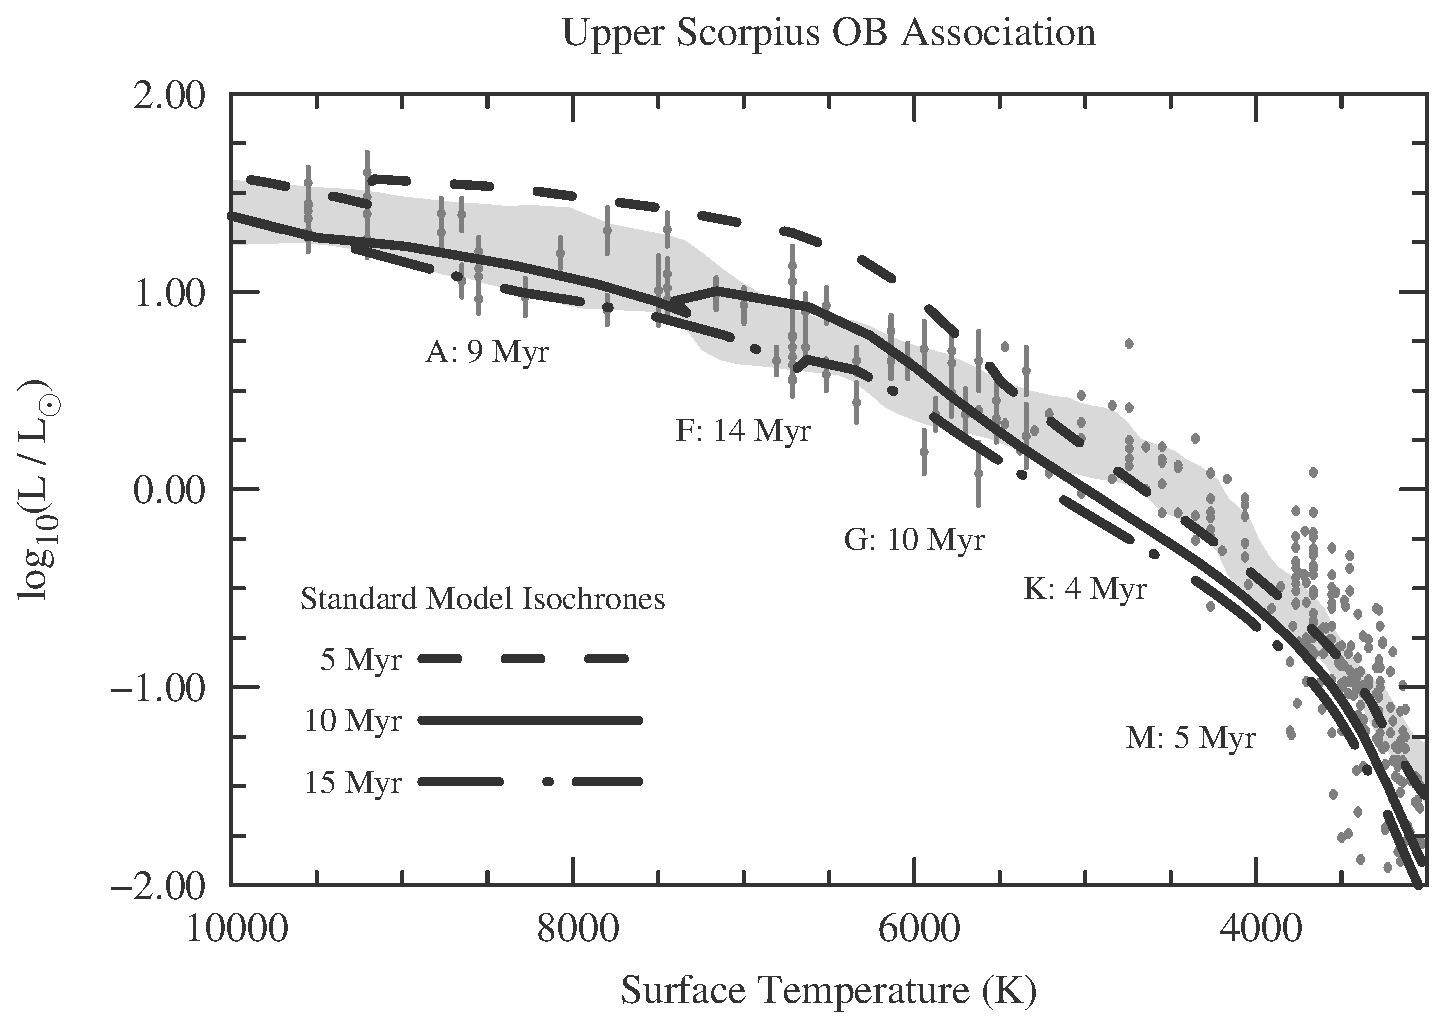
\includegraphics[width=0.65\columnwidth]{fig/USco_Age_Problems.eps}
	\caption{HR diagram for the Upper Scorpius OB Association. Stellar evolution model isochrones are shown in black. Labels show the ages inferred from different sub-populations in the association, highlighting a clear discordance between ages of hot and cool stars.}
	\label{fig:badhrd}
	\vspace{-0.2in}
\end{figure}

The difficulty is identifying which physics are missing from the models. Several mechanisms have been proposed to explain the luminosity spreads observed in HRDs of the youngest clusters. Examples include episodic accretion \citep{Baraffe2009, Baraffe2010} and starspots \citep{Somers2015b}, which can cause intrinsic variations in luminosity among a coeval population of stars. Until recently, there had not been a convincing demonstration of a physical mechanism to explain the observed effective-temperature-dependent ages or to explain the discrepancies between HRD and MRD age estimates. There had only been speculation that was focused on the usual suspects that are blamed for uncertainties in stellar models: convection, radiative opacities, or the absence of magnetic fields and starspots  \citep{Stassun2014, Soderblom2014, Herczeg2015}. 

% without supporting evidence





%{\bf\large 2. Previous Work: Magnetic Fields in Early Stellar Evolution} \addcontentsline{toc}{section}{Previous Work: Magnetic Fields in Early Stellar Evolution} 
%
%
%\citet{DAntona2000} presented the first hints the missing physics, well before the full severity of model deficiencies was understood. They showed that including a rudimentary prescription for the effects of magnetic fields on convection provided better...

\begin{figure}
	\centering
    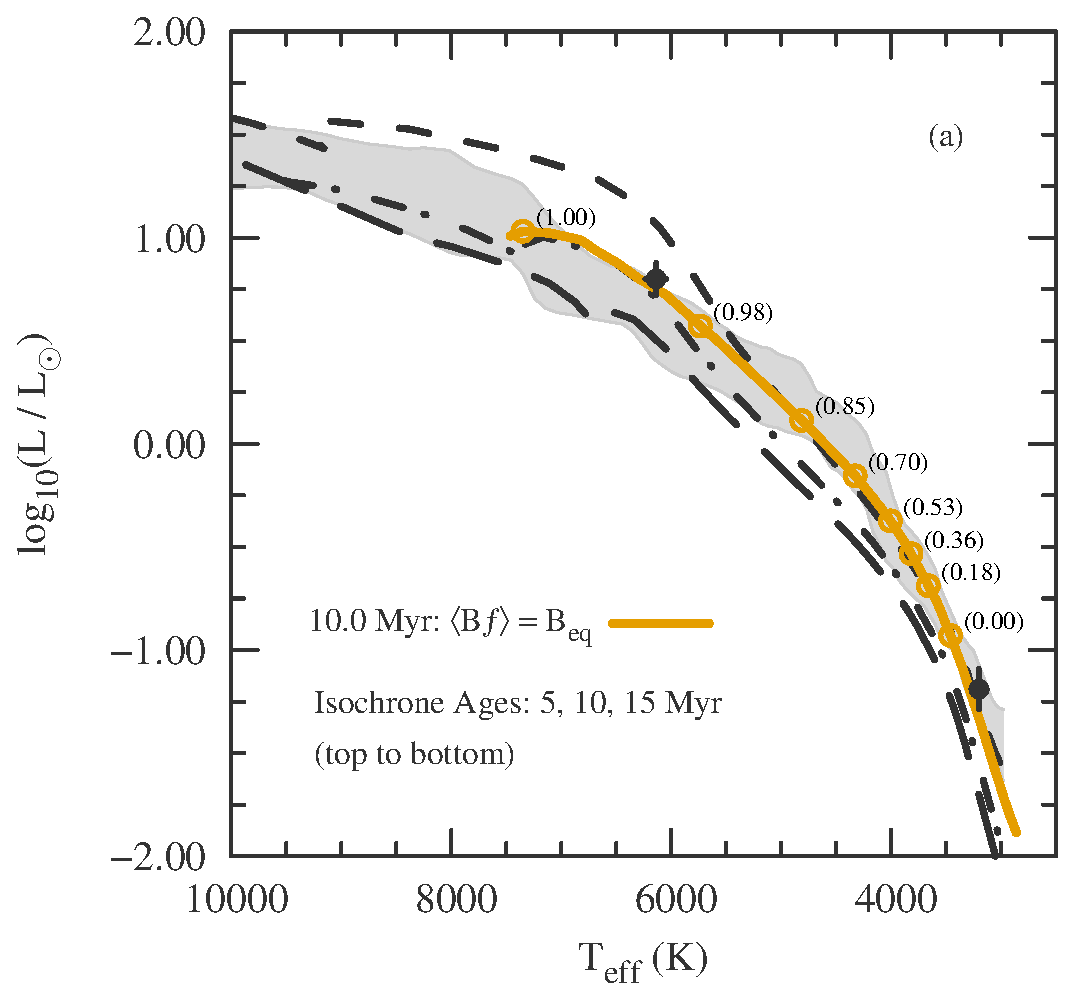
\includegraphics[scale=0.45]{fig/USco_HR_diagram.eps} \hspace{\fill}
    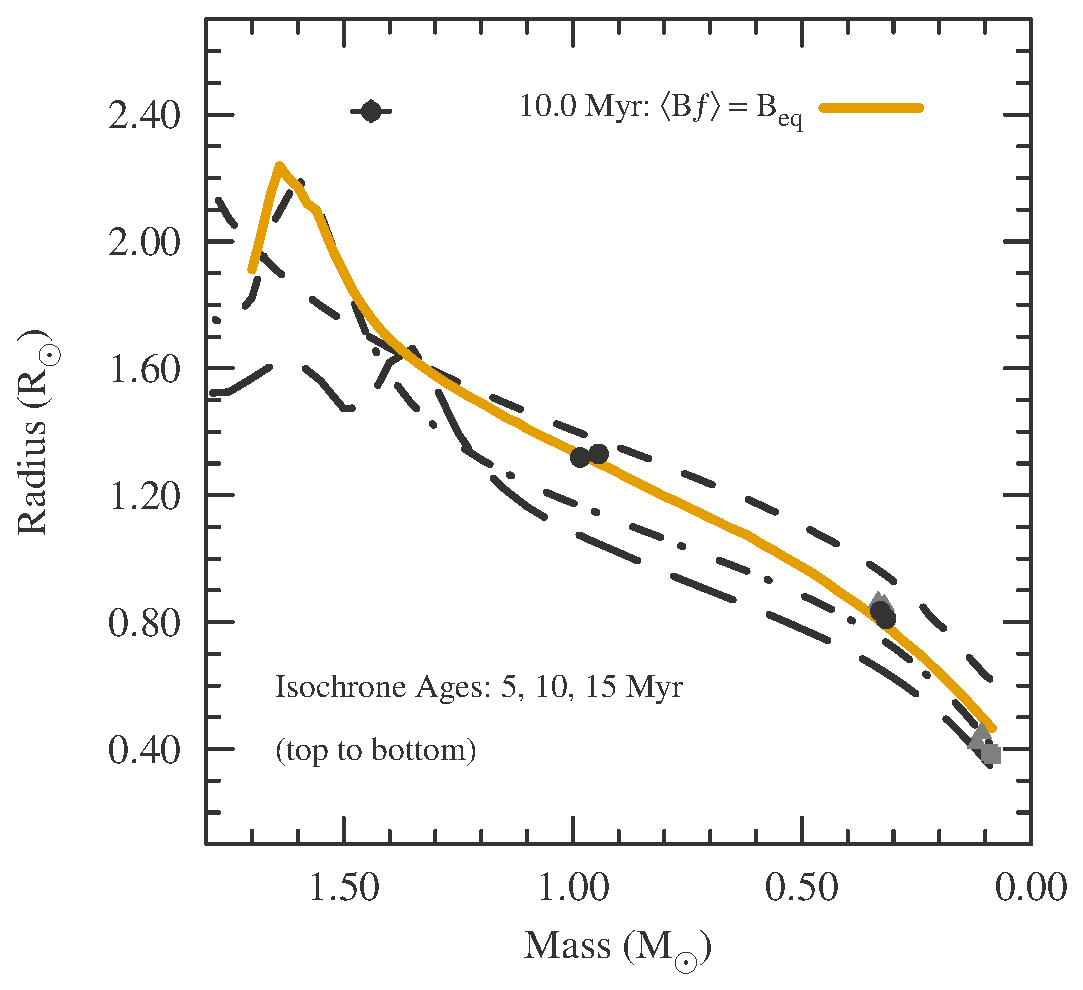
\includegraphics[scale=0.45]{fig/USco_MR_diagram.eps}
    \caption{({\it left}) HR diagram of Upper Scorpius with components of eclipsing binary systems UScoCTIO5 \citep{Kraus2015} and HD 144548 \citep{Alonso2015}
    observed by {\it Kepler}/K2 (black points). A 10 Myr magnetic stellar evolution isochrone is shown by the solid blue line. Note that the 10 Myr magnetic isochrone lies on top of the 5 Myr standard isochrone. ({\it right}) Mass-radius relationship for Upper Scorpius from {\it Kepler}/K2 eclipsing binary systems. {\it Unlike standard models, magnetic stellar evolution models naturally reproduce the slope of the low-mass mass-radius relationship at the same age predicted from the HR diagram.}}
    \label{fig:usco}
    \vspace{-0.2in}
\end{figure}

Recently, our group demonstrated that magnetic fields may provide a viable explanation for observed surface-temperature dependent ages in young clusters and the discordance between HRD and MRD age estimates \citep[see Figure~\ref{fig:usco};][]{Feiden2016}. The hypothesis is that Lorentz forces generated by strong magnetic fields suppresses convective flows in young stars, which acts to cool the stellar surface \citep[e.g.,][]{DAntona2000, MM01, FC12b}. As a result, the contraction of young pre-main-sequence stars is delayed, meaning young stars have cooler temperatures and larger radii at a given age when magnetic inhibition of convection is included in model calculations \citep{MM10, Feiden2016}. The physical mechanism is analogous to formation of sunspots, where strong magnetic fields suppress convection causing the stellar plasma contained within a magnetic region to cool and thus appear darker than its surroundings \citep{Biermann1941, Deinzer1965}. The difference is that sunspots are highly localized phenomena whereas our models consider global-scale magnetic inhibition of convection. 

Previous investigations showed that magnetic inhibition of convection could relieve age disparities between HRD ages and lithium depletion boundary ages \citep{DAntona2000}. For examples, ages inferred from an HRD for cool star members of the $\beta$ Pictoris moving group using standard stellar evolution models indicated the group was 10 Myr old \citep{Zuckerman2001}, while the same models provided an age of 20 Myr based on the lithium depletion boundary location \citep{Song2002, Binks2014}. However, by including magnetic inhibition of convection, \citet{MM10} and \citet{Malo2014} showed that the two age estimates could be brought into rough agreement at an age of 25 -- 30 Myr. Shortly thereafter, \citet{Mamajek2014} re-derived an age for high-mass members of the $\beta$ Pictoris moving group and found an age consistent with the magnetic model predictions for the ages of the cool stars. This provided the first hint that magnetism may explain effective-temperature-dependent ages.
%age discrepancies for the 25 Myr old $\beta$ Pictoris moving group \citep{MM10, Malo2014}.

Magnetic models were successful at reconciling the two age estimates, but it was not clear whether the magnetic models were {\it accurate} because HRD and lithium depletion boundary studies are mass agnostic. To know whether magnetic models predict accurate properties for real stars, EBs in well-studied young clusters were needed. Masses and radii directly measured for stars in EBs provide the most stringent test of stellar models as mass is the primary model input and observationally determined radii are more reliable than $T_{\rm eff}$ and luminosity estimates. Finding EBs in young clusters would also provide an opportunity to confirm the MRD age estimate against an age inferred from an HRD using an independent sample of stars.

A source of EBs in a well-studied young cluster became available when \kepler\ observed the Scorpius-Centaurus OB Association for 80 continuous days. A number of EBs were quickly identified in the Upper Scorpius subgroup, including two EBs for which precise masses and radii were determined \citep{Kraus2015, Alonso2015}. Critically, the two EBs occupied two distinct regions of the MRD thereby defining a preliminary mass-radius relationship (see Figure~\ref{fig:usco}). Comparing the EB mass-radius relation against model predictions, it is clear that standard models predict an incorrect {\it slope} for the mass-radius relationship. Ultimately, models were found to exhibit errors in age by up to 100\% and using the empirical HRD to derive a mass from standard models yields errors in the true mass by up to 50\% \citep{Kraus2015}.

However, when we compare the mass-radius relationship predicted by models that include magnetic inhibition of convection, we find that the model mass-radius relation steepens such that it closely matches the observed relationship at an age of approximately 10 Myr \citep[see Figure~\ref{fig:usco};][]{Feiden2016}. Figure~\ref{fig:usco} also demonstrates that the age predicted by the magnetic models in the MRD provides a reasonable fit to the median HRD sequence. {\bf Magnetic models appear to predict a consistent age in both the HRD and MRD. Furthermore, magnetic models predict an age that is largely independent of effective temperature in the HRD.} What's more, is that the surface magnetic fields strengths used to compute the stellar models were selected {\it a priori} based on arguments that the magnetic field is in thermal equipartition with the surrounding gas, as has been observed among young T-Tauri stars \citep{JohnsKrull1999}, and deep interior magnetic field strengths are of a plausible magnitude \citep{Browning2016}. This means magnetic models are exhibiting some level of predictive power when it comes to reproducing the properties of young stars.

% \citep{JohnsKrull1999}. 
%Results from \citet{Feiden2016} are tantalizing, as they offer a path toward reliable young stellar ages, but important questions remain about the validity and accuracy of these ``magnetic stellar evolution models.'' First, properties of the magnetic field are prescribed in a rather ad-hoc fashion \citep{FC12b, FC13}. Simple functions are used to describe the magnetic field strength as a function of radius deep in a star \citep{FC13}, but the situation in real stars is far more complex and depends intimately on the precise structure and rotational velocity of the star \citep{Browning2008, Brown2010}. Second, the interaction of Lorentz forces on convection depend strongly on the magnetic field topology throughout the star \citep{FC13}. At the moment, models use a free parameter to describe an average magnetic field topology, but the parameter is fixed and not allowed to vary as would be expected for a real magnetic field \citep{FC12b}. Finally, the existing magnetic field framework requires the specification of the surface magnetic field strength \citep{FC12b}. This value is either chosen arbitrarily \citep{FC12b, FC13, FC14, FC14b}, or at best, order of magnitude estimates are used to describe a possible maximum value \citep{Feiden2016}. The latter estimates are consistent with field strengths observed on young T Tauri stars \citep{JohnsKrull1999}, but this provide only indirect support for the model predictions.

%The full effect of these modeling choices are felt when stars are allowed to evolve in time. Properties of the magnetic field are a function of the stellar structure and stellar rotation, which both vary over time. Therefore, magnetic fields are expected to also evolve in time. 

Results from \citet{Feiden2016} are tantalizing, as they offer a path toward reliable young stellar ages, but important questions remain about the validity and accuracy of these ``magnetic stellar evolution models.'' Answers to some of these questions, such as whether model predict the correct mass-radius relationship across the entire MRD, are near at hand thanks to immense efforts to uncover and characterize EBs in young stellar populations with \kepler. However, detailed studies testing new hypotheses, such as magnetic inhibition of convection, are currently hampered by a lack of availability of models that incorporate these new physics (e.g., accretion, magnetic fields, starspots). To make real progress in understanding the observed discrepancies, theoretical models must be available to permit quantitative tests of predictions made by new models. \\


 
%a grid and tools to facilitate adoption of standard and magnetic models is needed to provide a means of testing and magnetic hypothesis.



%

\phantomsection
{\bf\large 2. Program Proposal: A Grid of Early (sub)Stellar Evolution Models with Magnetic Fields} \addcontentsline{toc}{section}{Program Proposal: A Grid of Early (sub)Stellar Evolution Models with Magnetic Fields} 

{\bf We propose to create a large, publicly available grid of standard and magnetic (sub)stellar evolution models along with tools to facilitate their adoption by the community.} Our finely sampled grid will cover a wide range in mass, metallicity, and surface magnetic field strength---including a sub-grid of models with an evolving magnetic field strength---yielding a total of approximately 130\,000 individual models. Model masses will extend from approximately $0.01\ M_{\odot}$ up to $6.0\ M_{\odot}$, for a total of 360 mass points with metallicities in the range of $-2.0\ {\rm dex}\le [m/H] \le +0.5\ {\rm dex}$ for a total of 20 metallicity values. Surface magnetic field strengths will range from $\langle {\rm B}f\rangle = 0.0$~kG (standard models) up to approximately $\langle {\rm B}f\rangle = 5.0$~kG. 

%Most observational studies of young stars assume solar metallicity, but some stars---such as those in $\beta$ Pic moving group---may have non-solar compositions \citep{Malo2014}.

The program will leverage the existing code base developed by PI Feiden. Stellar models will be calculated with the Dartmouth stellar evolution code \citep{Chaboyer2001, Bjork2006, Dotter2008}, which includes magnetic inhibition of convection \citep{FC12b}. Improvements to the code's microphysics are required to meet the grid specifications outlined above, notably for modeling objects below the nominal core hydrogen burning limit ($\sim 0.08\ M_{\odot}$). The magnetic version of the code is well tested \citep{FC12b, FC13, FC14, FC14b} and has been demonstrated to potentially relieve age discrepancies in young stellar populations \citep{Feiden2016}. 

In addition to the model grid, we will develop tools to create theoretical isochrones and to determine stellar parameters of real stars using Bayesian inference. The tools will be distributed as a standalone software package and as an online tool available through the user's web browser. Our isochrone software will allow a user to create stellar evolution isochrones from mass tracks available in the model grid and then determine the properties of young stellar populations (e.g., age, metallicity). Software to determine stellar parameters will permit users to specify a set of observed stellar properties (e.g., photometric magnitudes, \teff, bolometric flux, stellar mean density from exoplanet transit) and then determine the best fit stellar parameters (e.g., mass, radius, distance, metallicity, age) from stellar models with realistic statistical uncertainties \citep[see, e.g.,][]{Mann2016}. 

Software and analysis tools will also be based on existing code. An isochrone creation tool is partially written based on the principle of "equivalent evolutionary phases" \citep{Bergbusch1992, Dotter2016} and will extend the capabilities of tool distributed with the Dartmouth Stellar Evolution Database \citep{Dotter2008}. Stellar parameter determination will be performed using a Bayesian inference method. The code will be an updated and generalized version of the parameter inference software our team currently uses for stellar characterization \citep{Mann2015, Mann2016}. \\


\phantomsection
{\bf\large 3. Scientific Significance} \addcontentsline{toc}{section}{Scientific Significance} 

The stellar evolution model grid and associated analysis tools we intend to develop and distribute will permit more accurate determinations of absolute stellar ages and masses. Communities studying young stellar populations, star formation, planet formation, planetary system evolution, and characterizing exoplanets will strongly benefit from the availability of models that are able to more accurately reproduce the observed properties of real stars. Our model grid will therefore have a broad influence on a number of research areas, including:
\begin{itemize}
	\item {\bf Probing New Physics in Stellar Evolution:} There is ample evidence that standard stellar evolution models for young stars cannot reproduce the observed properties of real stars \citep[e.g.,][]{Hillenbrand2004, Soderblom2014, Stassun2014}. As mentioned in the Background, various hypotheses have been proposed to explain model shortcomings, including episodic accretion \citep[e.g.,][]{Baraffe2009}, magnetic inhibition of convection \citep[e.g.,][]{Feiden2016}, and starspots \citep[e.g.,][]{Jackson2009}. Future observing campaigns, such as the characterization of more young EBs, will continue to test the validity of standard stellar evolution models in an effort to quantify errors and reveal more about the nature of observed discrepancies \citep[e.g.,][]{Kraus2015}. However, greater progress will be made in assessing the physics important in early stellar evolution if those same observational campaigns are able to test theoretical predictions from state-of-the-art models incorporating aspects of the aforementioned hypotheses. \\
	
% A hallmark of many observational campaigns (e.g., studies of EBs) is comparing results to theoretical predictions. For stellar evolution models, this often involves overlaying model isochrones and/or mass tracks on the data and performing a by-eye comparison in the HRD or MRD. Models predictions are then either confirmed by to consistent or inconsistent with the observational data. If model predictions disagree with observations, speculations are made as to why models do not agree. More detailed studies testing proposed hypotheses are hampered by the lack of availability of models that incorporate new physics that may underlie the observed disagreements (e.g., accretion, magnetic fields, starspots). To make real progress in understanding the observed discrepancies, theoretical models must be available to permit quantitative tests of predictions made by new models (e.g., magnetic field strengths). ({\bf Coll. Kraus}) \\

	\item {\bf Characterization of Young Transiting Exoplanet Host Stars:} \kepler\ is revealing a number of transiting exoplanet candidates around stars in young stellar populations \citep[e.g,][]{Mann2016, Mann2016b, David2016}. The principle uncertainties in interpreting transit data are the properties of the host star (e.g., radius, mass, and age). Stellar radii are crucial for determining the radius of a transiting planet, as the transit depth is determined by the ratio of the planet's radius to the stellar radius. For young stars, one obtains consistent radii using standard and magnetic models, but the mass and age associated with the given radius are different by a factor of two (e.g., Mann et al. 2016 vs David et al. 2016). Accurate ages and masses are needed to help us understand the secular dynamical evolution of planetary systems (see below) and help us connect planet occurrence across cosmic time. ({\bf Colls. Mann \& Rizzuto})   \\
	
	\item {\bf Migration Timescale for Short-Period Exoplanets:} The dominant physical mechanism(s) responsible for producing short-period giant planets ($P_{\rm orb} < 20$ days) is currently unknown. Planets may form in-situ close their host star \citep{}, they may migrate through the protoplanetary disk \citep{}, or they may be subject to planet-planet interactions (Lidov-Kozai mechanism) that scatter planet into tight orbits about their host star \citep{}. Each process likely has an influence on the resulting short-period planet distribution observed around older stars (e.g., the original \emph{Kepler} sample), but which mechanism dominates the resulting distribution is uncertain. Since the aforementioned mechanisms each occur over different timescales, the key to identifying the dominant mechanism is to trace the occurrence of short-period planets around stars of similar masses in clusters with a large range in ages. Therefore, it is critical to obtain accurate masses for individual stars and accurate ages for their host cluster. ({\bf Colls. Rizzuto \& Mann})\\
	
	\item {\bf Masses of Directly-Imaged Substellar Objects:} Directly-imaged substellar companions provide important constraints on the shape of the brown dwarf and giant planet initial mass function \citep[e.g.,][]{Chabrier2003}. The initial mass function for these objects informs our understanding about how brown dwarf and giant planet form and whether the physical mechanisms are similar for these two classes of objects \citep{Chabrier2014}. A large number of directly-imaged substellar objects are now being uncovered \citep[e.g.,][]{Chauvin2004, Kalas2008, Spiegel2011, Bower2013, Hinkley2015, Macintosh2015}, but the key to interpreting the observations is knowing the host star's age. This is because substellar objects cool over time, meaning their brightness contrast and spectra also change over time. Errors in the host star's age at the 50\% level, as is currently the case for ages predicted by low-mass stellar models, introduces an error in mass estimates of a factor of 2 for objects near the deuterium burning limit \citep{Chabrier2000} and upward of a factor of 5 for Jupiter mass objects \citep{Baraffe2003}. Furthermore, if magnetic fields are able to delay the contraction timescale for young substellar objects, this introduces potential systematic errors in mass estimates of order 25\%, on top of the errors introduced by age corrections \citep{Chabrier2000}.  \\
	
	\item {\bf Giant Planet Formation Timescales:} A critical ingredient for giant planet formation theory is the time during which gas is available in primordial circumstellar disks. Surveys of gaseous circumstellar disks around stars in young clusters indicate that the fraction of stars with primoridal gas disks decreases over time \citep{Haisch2001, Mamajek2009}, placing an upper limit on the time during which giant planets must form. Giant planet formation theories indicate that the number of giant planets that form around young stars is a extremely sensitive to this timescale. Current estimates suggest the half-life for primordial gas disks is about 2 - 5 Myr \citep[e.g.,][]{Mamajek2009}. Planet formation theories struggle to properly form giant planets within this timeframe \citep{}. However, most current estimates are based on cluster ages inferred from standard stellar evolution models that are subject to significant age errors, suggesting the giant planet formation timescale may be longer. Recent estimates suggest the timescale may be upward of 20 Myr \citep{Bell2013}. \\
	
	\item {\bf Star Formation History:} Empirical HRDs of young stellar clusters in the Milky Way and the Large and Small Magellanic Clouds exhibit significant luminosity spreads for stars with a given $T_{\rm eff}$ \citep[e.g.,][]{Hillenbrand1997, DaRio2010b, DaRio2010a}. Luminosity spreads are often invoked as evidence of intrinsic age spreads in young clusters, suggesting that star formation is a prolonged process \citep{Hillenbrand1997}. This interpretation is in conflict with theoretical descriptions of star formation, which suggest star formation is a relatively rapid process \citep{Elmegreen2000}. It is possible that magnetism can partially explain the luminosity spread \citep[via starspots;][]{Somers2015b}, but robust age estimates are still required to evaluate the maximum possible age spread in a cluster. If stars are affected by magnetic inhibition of convection, age estimates may uniformly increase by as much as 100\%. ({\bf Coll. Johnson}) \\
	
	\item {\bf Universality of the Stellar IMF:} The stellar initial mass function (IMF) is a cornerstone of modern astrophysics and has historically been assumed to be independent of galactic environment. However, there are suggestions from extragalactic studies that the IMF is not universal and may be either top-heavy \citep{} or bottom-heavy \citep[e.g.,][]{vanDokkum2012} depending on the galactic environment. Even in the Milky Way, there is suggestion of a bottom-heavy IMF for the Taurus-Auriga association, which shows a relatively large number of low-mass stars for the observed population of high-mass stars \citep{Luhman2009}. The greatest systematic uncertainty in IMF studies is the conversion from observational properties to masses, which necessarily rely on stellar evolution models. As discussed above, errors in standard stellar model mass predictions are upward of 50\%, but magnetic models can relieve these mass discrepancies. \citet{Feiden2016} also showed that there exists a transition region where magnetic inhibition of convection weakens, which causes stars in a narrow mass range to be spread more widely across an HRD as compared to predictions from standard models. ({\bf Coll. Kraus \& Johnson}) \\

\end{itemize}



\phantomsection
{\bf\large 4. Relevance to NASA Programs \& Missions} \addcontentsline{toc}{section}{Relevance to NASA Programs \& Missions} 

Stellar evolution models of young stars are known to exhibit significant inaccuracies, with errors of order 50\% in mass and 100\% in age. Yet, a large number of other areas in astrophysics rely heavily on predictions from stellar evolution models at young ages. Our project provides a path toward relieving these inaccuracies and supplies state-of-the-art models to act as a foundation for interpreting an array of astronomical observations. {\bf In particular, our program will support two strategic programs for NASA's Astronomy Division: the Cosmic Origins and Exoplanet Exploration programs.}

{\bf 4.1 Cosmic Origins}

A key objective in the Cosmic Origins program is to understand the mechanisms involved in star formation. One of the fundamental predictions of star formation theory is the stellar initial mass function (IMF). Observational determination of the stellar IMF relies almost exclusively on stellar evolution models to translate observed properties of real stars (e.g., photometric magnitudes and colors) into a stellar mass. At the moment, erroneous mass predictions from stellar models represents a significant uncertainty in IMF determinations. 

{\bf 4.2 Exoplanet Exploration}

Our program will provide state-of-the-art for the characterization of transiting exoplanet host stars revealed by \kepler\ and the future TESS mission. Combining our models with our stellar parameter inference tool, we will provide reliable stellar masses, radii, and ages for host stars in young stellar clusters with statistical uncertainties. The capability of our approach has already been demonstrated in the Zodiacal Exoplanet in Time (ZEIT) program ({\bf Colls. Mann \& Rizzuto}). 

{\bf 4.3 Current \& Future NASA Missions}

{\it 4.3.1 \kepler}

As mentioned above, properties of exoplanets are discovered by \kepler\ are intimately tied to their host star's properties. Determining stellar masses, radii, and ages is typically a role left for stellar evolution models. An exciting development with \kepler\ is the study of young clusters, where standard stellar models are known to be inadequate. Models from our program will help alleviate significant uncertainties in the determination of stellar (and thus planetary) parameters, particularly stellar ages, which are crucial for tracing planetary system architectures through time.

Furthermore, \kepler\ is discovering an extraordinary number of EBs. An objective of many EB studies is to test and calibrate stellar evolution models. There is ample evidence that models fail to reproduce the properties of young stars in EBs \citep[see, e.g.,][]{Stassun2014}. While there are several hypotheses as to why this is the case, no model sets exist to provide EB observers with an opportunity to test new hypotheses. Our program will allow EB researchers to advance stellar evolution by testing the magnetic field hypothesis and testing the latest stellar model predictions. ({\bf Coll. Kraus}) 

{\it 4.3.2 James Webb Space Telescope (JWST)}

The JWST is set to provide space-based near- to mid-infrared (NIR to MIR) imaging and NIR spectroscopic capabilities that will undoubtedly reveal the presence of proto-planetary disks around a number of young stars. To understand how proto-planetary disks evolve with time, it's essential to have reliable estimates of the host star's age. Our program will able to provide age estimates for isolated young stars and stars in young moving groups, enabling a reliable interpretation about how proto-planetary disks evolve with time.

{\it 4.3.3 Transiting Exoplanet Survey Satellite (TESS)}

The future TESS mission is designed to observe the nearest and brightest stars to monitor their brightness for signatures of planetary transits \citep{Ricker2014}. A number of the stars observed by TESS are likely to be bright young stars. Coupled with parallax and proper motion data from \emph{Gaia}, our models will be able to identify young stars and provide estimates of the stellar properties, particularly the age. As with \kepler, our models will thus be a viable source of stellar parameters for transiting exoplanet host stars observed by TESS. \\


\phantomsection
{\bf\large 5. Technical Plan} \addcontentsline{toc}{section}{Technical Plan} 

There are two distinct components to our program: development of the (sub)stellar evolution model grid and development of the tools necessary to facilitate their distribution and adoption throughout the community. 

{\bf 5.1 (Sub)Stellar Evolution Model Grid}

{\it 5.1.1 Surface Boundary Conditions \& Model Atmosphere Structures}

Stellar evolution models require specification of surface boundary conditions, typically taken to the pressure and temperature at a given optical depth. The Dartmouth stellar evolution code uses thermal structures from stellar model atmosphere calculations to extract $P_{\rm gas}$ and $T_{\rm gas}$ at an optical depth $\tau_{\rm Ross} = 10$ using $T_{\rm eff}$, [$m$/H], and \logg\ to define the appropriate atmosphere model \citep{Feiden2016}. Currently, the Dartmouth code uses PHOENIX AMES-COND model atmospheres \citep{Hauschildt1999a} for cool stars ($T_{\rm eff} > 10\,000$~K and ATLAS model atmospheres for hot stars \citep{Castelli2004}. However, we recently discovered that the original PHOENIX models have an erroneous thermal structure at optical depths $\tau > 1$, suggesting revisions to models may be required. This also creates a situation where the transition from PHOENIX to ATLAS surface boundary conditions at high optical depths is not smooth, causing models to crash. 

%%% FIGURE: MISMATCH/ERRORS WITH ORIGINAL MODEL ATMOSPHERES?

Unfortunately, we cannot simply adopt a single model atmosphere model to prescribe surface boundary conditions: PHOENIX models no longer compute models with the \citet{GS98} solar composition and ATLAS does not have grid available for more recent solar compositions \citep[e.g.,][]{Asplund2009}. For consistency, it is desirable to maintain the same input physics throughout our full model grid, meaning we should not in one instance adopt only PHOENIX models \citep[for][]{Asplund2009} and in another adopt a mix of PHOENIX and ATLAS \citep[for][]{GS98}.

To overcome these issues, we are computing new grids of model atmospheres to use as surface boundary conditions for stars with $T_{\rm eff} > 2\,800$~K and for deriving new synthetic color-$T_{\rm eff}$ relations with updated atomic and molecular line lists \citep{Plez2012}. We will use a combination of PHOENIX \citep{Allard2011}, MARCS \citep{Gustafsson2008}, and ATLAS \citep{Castelli2004} model atmospheres for $T_{\rm eff} < 2\,800$~K, $2\,800 \textrm{ K} \le T_{\rm eff} < 8\,000$~K, and $T_{\rm eff} \ge 8\,000$~K, respectively. MARCS and ATLAS use similar physics in the vicinity of $T_{\rm eff} \approx 8\,000$~K, so there should be no loss of consistency. For $T_{\rm eff} \approx 3\,000$~K, there is little difference between model atmosphere structures from PHOENIX and MARCS \citep{Gustafsson2008}, meaning there should also be a minimal loss of consistency at lower temperatures (see below).

{\it 5.1.2 Extending Dartmouth Models to Lower Masses}

The Dartmouth stellar evolution code is currently optimized to model stars with masses between $0.1 \lesssim M/M_{\odot} \le 6.0$. The lower mass limitation is imposed by the validity of the adopted gas equation of state and surface boundary conditions. Currently, we use the FreeEOS \citep{Irwin2007}, which is not designed to model cool, high pressure environments characteristic of the outer layers in brown dwarfs \citep{Chabrier2000}. To overcome this limitation, we will use the \citet{scvh95} equation of state. The equation of state is already incorporated into the Dartmouth code, but is currently not operational as it was not properly maintained over the years. We will enable this equation of state and compare model results in the vicinity of $0.1\ M_{\odot}$ to ensure consistency with the rest of the grid computed with FreeEOS.

Surface boundary conditions used by the original Dartmouth stellar evolution code are valid down to $T_{\rm eff} \approx 2\,700$~K \citep{Hauschildt1999a}. Our current \citep{Hauschildt1999a} and future \citep{Gustafsson2008} model atmospheres do not treat dust species, which begin to form below $T_{\rm eff} \approx 2\,700$~K. The Dartmouth code has since been updated to include the latest PHOENIX BT-Settl model atmospheres \citep{Allard2011} that attempt to treat the formation of dust within the gas equation of state and radiative opacities. As mentioned above, in the transition region between where we will use MARCS and PHOENIX models, the two model sets produce similar thermal structures and therefore do not significantly influence the resulting interior model calculation. Nevertheless, we will compare interior model results using PHOENIX and MARCS boundary conditions to ensure consistency of model predictions across this boundary.

{\it 5.1.3 Evolving Magnetic Field}

%%%% FIGURE: EVOLUTION OF MAGNETIC FIELD WITH TIME?

Stellar evolution models that include magnetic inhibition of convection (Delaware code, Mullan \& MacDonald 2001; Dartmouth code, Feiden \& Chaboyer 2012) are designed such that a surface magnetic field strength must be specified prior to calculating a model star. This value is typically adjusted as a free parameter until models reproduce empirical data \citep[e.g., radii of stars in EBs;][]{FC12b, FC13, FC14, MM14}. For work attempting to identify whether magnetic fields provide a viable explanation for anomalous properties of stars, this tactic is sufficient, as it yields a quantitative prediction for the surface magnetic field strength that can in principle be tested by observations. 

However, this approach is insufficient when comparing magnetic models against empirical HRDs and CMDs for stellar populations. This is because not all stars in a stellar population will have precisely the same magnetic field strength. Stars with different masses are likely to have different magnetic field strengths at a given age. Furthermore, the magnetic field strength for a star of a given mass changes over time, due to a combination of changing conditions at the stellar photosphere \citep[see, e.g.,][]{Feiden2016} and changes in stellar rotation \citep[e.g.,][]{Skumanich1972}. To model stellar populations, we therefore need a set of models that automatically prescribe the surface magnetic field strength as a function of stellar mass and age. 

In lieu of a stellar model with a complete magnetic dynamo mechanism, our next best estimate for young stars is assuming they have surface field strengths equal to their thermal equipartition value \citep{JohnsKrull1999}. This was shown to be a very reasonable {\it a priori} approximation by \citet{Feiden2016}, although their model surface magnetic field strengths did not evolve in time. We have developed a method by which the surface magnetic field strength is automatically determined based on thermal equipartition estimates as the model evolves in time. The method is already implemented in the Dartmouth code, but requires further testing to ensure models are converging and that they are numerically stable during their evolution. 

{\it 5.1.5 Computing the Model Grid}

Computation of the model grid is a core component of the project. Calculating of order 130\,000 individual models requires approximately 22\,000 CPU hours. These calculations will be performed on a multi-core desktop, which is equipped with two processors with six cores each (12 total cores) and 3 TB of hard disk capacity. On this machine, the computation of the model grid can be completed within 90 days, or the duration of an undergraduate summer project. The hard disk space is sufficient to store all data products for the full model grid. Various sub-grids have already been computed by PI Feiden, so the actual computation time required for the project will be less than 3 months. Results will be continually monitored to check for models that did not converge and ones that terminated pre-maturely.

Calculating new models is simplified with software that automatically generates all of the necessary input data for a stellar evolution model. While it may seem trivial, it is critical that an undergraduate can quickly learn how to run the stellar evolution code and generate new models so that the project can be accomplished within the time allotted. This software ensures that this is the case. Small modifications to the software need to be made to streamline organization of completed models, but it is otherwise complete.


{\it 5.1.6 Photometric Magnitudes and Colors}

After completion of the full model grid, a color--$T_{\rm eff}$ transformation will be applied to each model to convert their $T_{\rm eff}$, [$m$/H], \logg, and luminosity into synthetic absolute magnitudes and colors. We will compute synthetic photometry in standard Johnson-Cousins, 2MASS, HST WFC3 and ACS, {\it Gaia} BP/RP, \kepler, and TESS passbands. At the same time, we will distribute software to allow for the computation of other standard photometric passbands (e.g., SDSS) and also user-supplied passbands. Color--$T_{\rm eff}$ transformation will be applied using tables of bolometric corrections computed from the same model atmosphere structures used to specify surface boundary conditions \citep[see above;][]{Allard2011, Gustafsson2008, Castelli2004}.

{\it 5.1.7 Publicly Accessible Model Archive}

Stellar models computed for this program will be made publicly available online through a University of North Georgia web server. A simple, intuitive webpage will be constructed to allow users to quickly locate and download data products. Each individual stellar model produces two principle output files (one summary, one detailed) with information about how stellar model properties evolve with time (mass tracks). Synthetic photometry will be appended to the summary mass track. In addition, each individual model yields numerous snapshots that provide detailed information about the internal structure of a model at a given age. All data products from the stellar evolution models will be distributed as individual files and larger archive files containing portions of the full model grid. A single archive file with the full grid will also be made available.  

\begin{figure}[t]
	\centering
	\includegraphics[width=0.45\linewidth]{./fig/KJK.eps} \hspace{\fill}
	\includegraphics[width=0.45\linewidth]{./fig/smc_iso_cmd.pdf}
	\caption{Color-magnitude diagrams (CMDs) for ({\it left}) the Upper Scorpius OB Association and ({\it right}) the Small Magellanic Cloud (SMC). }
	\label{fig:smc}
	\vspace{-0.2in}
\end{figure}

{\it 5.1.8 Effects of Magnetic Inhibition of Convection on Stellar Properties}

The influence of magnetic inhibition of convection on the fundamental properties of young stars is generally understood. For a given mass star, models predict that magnetic inhibition of convection cool the stellar surface and delay pre-main-sequence contraction \citep{DAntona2000, MM10, Malo2014, Feiden2016}. While the basic picture about how magnetic fields affect young stellar model predictions is believed to be understood, details about how magnetic inhibition affects stellar interior structure in young stars  has been relatively unexplored \citep[e.g., on radiative core development;][]{Feiden2016}. With our large grid of magnetic models, we will systematically examine how stellar interior structure is affected by magnetic inhibition of convection and how the influence of magnetic fields changes with age and metallicity. We will evaluate the impact of the resulting interior structure changes on predicted lithium depletion curves \citep[see, e.g.,][]{Malo2014} and possible influences on asteroseismic oscillations \citep{Zwintz2014}.


{\it 5.1.9 Model Validation}

As we mentioned above, a grid of magnetic early stellar evolution models opens up the possibility for EB researchers to rigorously test the magnetic field hypothesis. We are running a program (PI Kraus) to characterize young EBs discovered by \kepler\ with this goal in mind. We have flagged 15 EBs in the 10 -- 20 Myr Scorpius-Centaurus OB Association. Crucially, the EBs are spread across the association's CMD, meaning a nearly complete mass-radius relationship can be formed and the validity of magnetic stellar models can be rigorously tested across a wide range of masses. One EB system has been published \citep[UScoCTIO 5;][]{Kraus2015}, which subsequently anchored the mass-radius relationship at the low-mass end and provided evidence to suggest that magnetic inhibition of convection may be an important factor in pre-main-sequence stellar evolution \citep{Feiden2016}. In addition, we are obtaining high-resolution near-infraread spectra using the IGRINS spectrograph ($R = 40\,000$) on the McDonald Observatory 107-in telescope. These spectra will allow us to measure strong surface magnetic field strengths on stars in the Scorpius-Centaurus OB Association via Zeeman splitting of spectral lines, providing a direct test of model magnetic field strength predictions.

Observations of EBs in the Scorpius-Centaurus OB Association provides validation of model predictions in a near-solar metallicity environment \citep{}. To test the accuracy of our models in a non-solar metallicity environment, we are running a program (PI Johnson) to compare standard and magnetic stellar evolution isochrones to CMDs of young clusters in the Small Magellanic Cloud (SMC; [$m$/H]~$\approx -0.75$) as part of the HST program ``The Small Magellanic Cloud Investigation of Dust and Gas Evolution (SMIDGE).'' We have high resolution, multi-band HST photometry of a region of the SMC that contains numerous young clusters. We will explore whether we observe similar modeling errors in SMC clusters as we do in Milky Way clusters and whether magnetic inhibition of convection is able to provide a viable solution to the observed modeling errors. Initial results indicate that models describe the morphology of young SMC clusters with reasonable accuracy, including possibly revealing the deuterium burning bump at the youngest ages, as shown in Figure~\ref{fig:smc}. 

{\bf 5.2 Supporting Analysis Tools}

A software package will be made available to access, manipulate, and run analyses with models contained in our grid. The code will be open source and version controlled using GitHub. There are two main components of our software package: the isochrone construction kit and the stellar parameter inference tool. 

{\it 5.2.1 Isochrone Construction Kit}

The primary output from a stellar evolution code is individual mass tracks, describing how a star of a given mass evolves over time. However, a number of applications of stellar evolution models (e.g., cluster age determinations) require the use of stellar model isochrones, which describe stellar properties as a function of mass at a given age. Constructing isochrones from mass tracks can be a notoriously tricky problem, particularly when attempting to describe advanced evolutionary stages \citep[see, e.g.,][]{Bergbusch1992, Dotter2016}. Therefore, it is customary for modelers to provide a grid of stellar model isochrones and interpolation routines. This becomes cumbersome for large model grids, especially because researchers want different age resolutions, meaning they must anyway download software and create new isochrones via interpolation. Instead of providing extensive isochrones, we will supply software to allow the user to generate their own sets of isochrones. This is only possible because we are committed to publishing and distributing all data products from our stellar evolution code. The isochrone routine will be based on a now-standard procedure of defining equivalent evolutionary phases \citep[EEPs;][]{Bergbusch1992}. Our isochrone software is partially completed, but it must be debugged, optimized, and incorporated into the larger software package.

{\it 5.2.2 Stellar Parameter Inference Tool}

Stellar evolution models are often used to determine fundamental parameters for single stars. To facilitate adoption of our models and promote rapid dissemination, we will provide software to compute best fit model parameters based on user supplied information about a real star. This software will be based on existing software currently used by the PI to determine stellar properties \citep{Boyajian2015, Mann2015, Mann2016, Gaidos2016}. Our current software uses a Markov Chain Monte Carlo (MCMC) method to sample the posterior probability distributions for the stellar parameters (mass, metallicity, age, distance, radius, etc.) by exploring the parameter space defined by a small existing grid of stellar models. The software determines model properties by using an N-dimensional interpolation routine, which is computationally expensive. Part of developing the parameter inference tool for public distribution will be to reduce computational costs by parametrizing the full N-dimensional grid using a number of polynomial relations to describe stellar properties as a function of mass, age, metallicity, and magnetic field strength. We must also generalize the code to accept an arbitrary set of observational data as input and automatically modify the likelihood function in the MCMC routine. In time we plan to make this tool available through an online web portal for users wishing to quickly determine model parameters for a single star. \\

\phantomsection
{\bf\large 6. Work Plan} \addcontentsline{toc}{section}{Work Plan}

Our program will be coordinated by PI Feiden at the University of North Georgia (UNG). The work will be largely conducted by PI Feiden and four undergraduate students from UNG, two of whom will be hired for summer 2017 and two hired for summer 2018.

{\bf 6.1 Plan for 2016}

The following work is set to be completed before the grant begins in 2017:

\begin{itemize}
	\item[] Feiden: Enable the \citet{scvh95} equation of state and test for consistency with the FreeEOS around 0.1 \msun. Finish implementing an evolving thermal equipartition surface magnetic strength routine. Test the evolving magnetic field strength routine to ensure the code is stable. Begin writing model grid paper number 1. \\
	
	\item[] Edvardsson: Compute opacity tables for two solar compositions for use in MARCS. \\
\end{itemize} 

{\bf 6.2 Plan for 2017}

\begin{itemize}
	\item[] Feiden: Compute grid of model atmospheres with GS98 solar composition. Supervise undergraduate researchers. Collaborate with Undergraduate 1 to analyze model results. Debug and optimize isochrone construction kit. Begin developing model grid archive website. Finish writing model grid paper number 1 (stellar fundamental properties). Begin writing model grid paper number 2 (synthetic photometry). \\
	
	\item[] Edvardsson: Compute grid of model atmospheres with AGSS09 solar composition. Compute tables with bolometric corrections as a function of \logg, [m/H], and \teff\ based on model atmospheres computed with GS98 and AGSS09 solar composition. \\
	
	\item[] Piskunov: Computation of ATLAS model atmospheres with AGSS09 composition. Test whether new atomic and molecular line lists affect model atmosphere thermal structure for models with GS98 composition. \\
	
	\item[] Kraus: Validation of model prediction by comparing standard and magnetic stellar evolution model predictions against the properties of EBs in young clusters revealed by \kepler. Focus on solar metallicity (galactic environments). \\
	
	\item[] Johnson: Validation of model predictions for young, metal-poor clusters in the Small Magellanic Cloud using multi-band photometry from HST. \\
	
	\item[] Undergraduate 1: Compute a large grid of stellar evolution models and check the resulting models for convergence. Organize model output data for distribution to the community. Computing customized models for Coll.\ Kraus's EB program, when necessary. Share role in analysis of model results in preparation for a paper describing the model grid. Help write model grid paper number 1. \\
	
	\item[] Undergraduate 2 [{\it preferably from UNG's mathematics department}]: Develop polynomial fits to stellar model mass tracks to succeed model grid interpolation. Generalize existing Bayesian parameter inference code using polynomial fits. Writing code documentation and tutorial(s). Write up polynomial fitting for future paper on software package. \\
\end{itemize} 

{\bf 6.3 Plan for 2018} 

\begin{itemize}
	\item[] Feiden: Integrate isochrone construction kit into software package. Continuing to develop model archive webpage. Computing custom models for Coll.\ Kraus's EB program, when necessary. Supervise undergraduate researchers. Finish writing model grid paper number 2. Write paper describing the analysis tools software package. \\
	
	\item[] Edvardsson: Finish computing tables with bolometric corrections based on model atmospheres computed with GS98 and AGSS09 solar composition.  \\
	
	\item[] Kraus: Continued comparison of standard and magnetic stellar evolution model predictions against the properties of EBs in young clusters revealed by \kepler. \\
	
	\item[] Mann: Testing and application of stellar parameter inference tool to compute stellar parameters for transiting exoplanet host stars uncovered by K2. \\
	
	\item[] Rizzuto: Testing and application of stellar parameter inference tool to compute stellar parameters for transiting exoplanet host stars uncovered by K2. \\

	\item[] Undergraduate 3: Finish software to compute synthetic photometry and integrate into larger software package. Compute synthetic photometry for complete stellar model grid. Compare theoretical CMDs to empirical CMDs from young clusters to evaluate model accuracy and derive ages for stellar clusters. Help write model grid paper number 2. \\
	
	\item[] Undergraduate 4 [{\it preferably from UNG's computer science department}]: Finish the stellar parameter inference tool and integrate into larger software package (if needed). Help develop webpage for model grid archive. Development of web portal for stellar parameter inference tool for online calculation of stellar parameters with statistical uncertainties. Help write paper on software package and web interface.
\end{itemize} 


\clearpage


\phantomsection
\renewcommand{\refname}{\bf\large 7. References}\addcontentsline{toc}{section}{7. References} 

\begin{thebibliography}{56}
\expandafter\ifx\csname natexlab\endcsname\relax\def\natexlab#1{#1}\fi

\bibitem[{{Allard} {et~al.}(2011){Allard}, {Homeier}, \&
  {Freytag}}]{Allard2011}
{Allard}, F., {Homeier}, D., \& {Freytag}, B. 2011, in Astronomical Society of
  the Pacific Conference Series, Vol. 448, 16th Cambridge Workshop on Cool
  Stars, Stellar Systems, and the Sun, ed. C.~{Johns-Krull}, M.~K. {Browning},
  \& A.~A. {West}, 91
  
\bibitem[{{Alonso} {et~al.}(2015){Alonso}, {Deeg}, {Hoyer}, {Lodieu}, {Palle},
  \& {Sanchis-Ojeda}}]{Alonso2015}
{Alonso}, R., {Deeg}, H.~J., {Hoyer}, S., {Lodieu}, N., {Palle}, E., \&
  {Sanchis-Ojeda}, R. 2015, \aap, 584, L8

\bibitem[{{Andersen}(1991)}]{Andersen1991}
{Andersen}, J. 1991, \aapr, 3, 91

\bibitem[{{Asplund} {et~al.}(2009){Asplund}, {Grevesse}, {Sauval}, \&
  {Scott}}]{Asplund2009}
{Asplund}, M., {Grevesse}, N., {Sauval}, A.~J., \& {Scott}, P. 2009, \araa, 1

\bibitem[{{Baraffe} \& {Chabrier}(2010)}]{Baraffe2010}
{Baraffe}, I., \& {Chabrier}, G. 2010, \aap, 521, A44

\bibitem[Baraffe et al.(2003)]{Baraffe2003} Baraffe, I., Chabrier, G., Barman, T.~S., Allard, F., \& Hauschildt, P.~H.\ 2003, \aap, 402, 701

\bibitem[{Baraffe {et~al.}(2009)Baraffe, Chabrier, \& Gallardo}]{Baraffe2009}
Baraffe, I., Chabrier, G., \& Gallardo, J. 2009, \apj, 702, L27

\bibitem[Bastian et al.(2010)]{Bastian2010} Bastian, N., Covey, K.~R., \& Meyer, M.~R.\ 2010, \araa, 48, 339

\bibitem[{{Bell} {et~al.}(2012){Bell}, {Naylor}, {Mayne}, {Jeffries}, \&
  {Littlefair}}]{Bell2012}
{Bell}, C.~P.~M., {Naylor}, T., {Mayne}, N.~J., {Jeffries}, R.~D., \&
  {Littlefair}, S.~P. 2012, \mnras, 424, 3178
  
\bibitem[Bell et al.(2013)]{Bell2013} Bell, C.~P.~M., Naylor, T., Mayne, N.~J., Jeffries, R.~D., \& Littlefair, S.~P.\ 2013, \mnras, 434, 806
  
\bibitem[Bergbusch \& Vandenberg(1992)]{Bergbusch1992} Bergbusch, P.~A., \& Vandenberg, D.~A.\ 1992, \apjs, 81, 163 

\bibitem[{{Biermann}(1941)}]{Biermann1941}
{Biermann}, L. 1941, Vierteljahresschrift der Astronomischen Gesellschaft, 76,
  194
  
\bibitem[Binks \& Jeffries(2014)]{Binks2014} Binks, A.~S., \& Jeffries, R.~D.\ 2014, \mnras, 438, L11

\bibitem[{{Bjork} \& {Chaboyer}(2006)}]{Bjork2006}
{Bjork}, S.~R., \& {Chaboyer}, B. 2006, \apj, 641, 1102

\bibitem[Bodenheimer et al.(1965)]{Bodenheimer1965} Bodenheimer, P., Forbes, J.~E., Gould, N.~L., \& Henyey, L.~G.\ 1965, \apj, 141, 1019

\bibitem[Bowler(2016)]{Bowler2016} Bowler, B.~P.\ 2016, PASP, in press; arXiv:1605.02731

\bibitem[{{Boyajian} {et~al.}(2015){Boyajian}, {von Braun}, {Feiden}, {Huber},
  {Basu}, {Demarque}, {Fischer}, {Schaefer}, {Mann}, {White}, {Maestro},
  {Brewer}, {Lamell}, {Spada}, {L{\'o}pez-Morales}, {Ireland}, {Farrington},
  {van Belle}, {Kane}, {Jones}, {ten Brummelaar}, {Ciardi}, {McAlister},
  {Ridgway}, {Goldfinger}, {Turner}, \& {Sturmann}}]{Boyajian2015}
{Boyajian}, T.~S., {von Braun}, K., {Feiden}, G.~A., {et~al.} 2015, \mnras, 447, 846

\bibitem[Browning et al.(2016)]{Browning2016} Browning, M.~K., Weber, M.~A., Chabrier, G., \& Massey, A.~P.\ 2016, \apj, 818, 189

\bibitem[{{Castelli} \& {Kurucz}(2004)}]{Castelli2004}
{Castelli}, F., \& {Kurucz}, R.~L. 2004, astro-ph/0405087

\bibitem[{Chaboyer {et~al.}(2001)Chaboyer, Fenton, Nelan, Patnaude, \&
  Simon}]{Chaboyer2001}
Chaboyer, B., Fenton, W.~H., Nelan, J.~E., Patnaude, D.~J., \& Simon, F.~E.
  2001, \apj, 562, 521

\bibitem[{{Chabrier}(2003)}]{Chabrier2003}
{Chabrier}, G. 2003, \pasp, 115, 763

\bibitem[{Chabrier {et~al.}(2000)Chabrier, Baraffe, Allard, \&
  Hauschildt}]{Chabrier2000}
Chabrier, G., Baraffe, I., Allard, F., \& Hauschildt, P.~H. 2000, \apj, 542,
  464

\bibitem[{Chabrier {et~al.}(2014)Chabrier, Johansen, Janson, \&
  Rafikov}]{Chabrier2014}
Chabrier, G., Johansen, A., Janson, M., \& Rafikov, R. 2014, Protostars and
  Planets VI, 619
  
\bibitem[Chauvin et al.(2004)]{Chauvin2004} Chauvin, G., Lagrange, A.-M., Dumas, C., et al.\ 2004, \aap, 425, L29

\bibitem[Chiang \& Laughlin(2013)]{Chiang2013} Chiang, E., \& Laughlin, G.\ 2013, \mnras, 431, 3444

\bibitem[Conroy \& van Dokkum(2012)]{Conroy2012} Conroy, C., \& van Dokkum, P.~G.\ 2012, \apj, 760, 71

\bibitem[{{Da Rio} {et~al.}(2010{\natexlab{a}}){Da Rio}, {Gouliermis}, \&
  {Gennaro}}]{DaRio2010b}
{Da Rio}, N., {Gouliermis}, D.~A., \& {Gennaro}, M. 2010{\natexlab{a}}, \apj,
  723, 166

\bibitem[{{Da Rio} {et~al.}(2010{\natexlab{b}}){Da Rio}, {Robberto},
  {Soderblom}, {Panagia}, {Hillenbrand}, {Palla}, \& {Stassun}}]{DaRio2010a}
{Da Rio}, N., {Robberto}, M., {Soderblom}, D.~R., {Panagia}, N., {Hillenbrand},
  L.~A., {Palla}, F., \& {Stassun}, K.~G. 2010{\natexlab{b}}, \apj, 722, 1092

\bibitem[D'Angelo et al.(2002)]{DAngelo2002} D'Angelo, G., Henning, T., \& Kley, W.\ 2002, \aap, 385, 647

\bibitem[{{D'Antona} {et~al.}(2000){D'Antona}, {Ventura}, \&
  {Mazzitelli}}]{DAntona2000}
{D'Antona}, F., {Ventura}, P., \& {Mazzitelli}, I. 2000, \apj, 543, L77

\bibitem[Dav{\'e}(2008)]{Dave2008} Dav{\'e}, R.\ 2008, \mnras, 385, 147

\bibitem[David et al.(2016a)]{David2016} David, T.~J., Hillenbrand, L.~A., Cody, A.~M., Carpenter, J.~M., \& Howard, A.~W.\ 2016, \apj, 816, 21

\bibitem[David et al.(2016b)]{David2016b} David, T.~J., Hillenbrand, L.~A., Petigura, E.~A., et al.\ 2016, Nature, 534, 658

\bibitem[{{Deinzer}(1965)}]{Deinzer1965}
{Deinzer}, W. 1965, \apj, 141, 548

\bibitem[Dotter(2016)]{Dotter2016} Dotter, A.\ 2016, \apjs, 222, 8 

\bibitem[{Dotter {et~al.}(2008)Dotter, Chaboyer, Jevremovi\'{c}, Kostov, Baron,
  \& Ferguson}]{Dotter2008}
Dotter, A., Chaboyer, B., Jevremovi\'{c}, D., Kostov, V., Baron, E., \&
  Ferguson, J.~W. 2008, \apjs, 178, 89
  
\bibitem[Elmegreen(2000)]{Elmegreen2000} Elmegreen, B.~G.\ 2000, \apj, 530, 277

\bibitem[Fabrycky \& Tremaine(2007)]{Fabrycky2007} Fabrycky, D., \& Tremaine, S.\ 2007, \apj, 669, 1298

\bibitem[{{Feiden}(2016)}]{Feiden2016}
{Feiden}, G.~A. 2016, \aap, in press; arXiv:1604.08036.

\bibitem[{{Feiden} \& {Chaboyer}(2012)}]{FC12b}
{Feiden}, G.~A., \& {Chaboyer}, B. 2012, \apj, 761, 30

\bibitem[{{Feiden} \& {Chaboyer}(2013)}]{FC13}
{Feiden}, G.~A., \& {Chaboyer}, B. 2013, \apj, 779, 183

\bibitem[{{Feiden} \& {Chaboyer}(2014{\natexlab{a}})}]{FC14}
{Feiden}, G.~A., \& {Chaboyer}, B. 2014{\natexlab{a}}, \apj, 786, 53

\bibitem[{{Feiden} \& {Chaboyer}(2014{\natexlab{b}})}]{FC14b}
{Feiden}, G.~A., \& {Chaboyer}, B. 2014{\natexlab{b}}, \aap, 571, A70

\bibitem[Gaidos et al.(2016)]{Gaidos2016} Gaidos, E., Mann, A.~W., Rizzuto, A., et al.\ 2016, arXiv:1606.05812 

\bibitem[{{Grevesse} \& {Sauval}(1998)}]{GS98}
{Grevesse}, N., \& {Sauval}, A.~J. 1998, \ssr, 85, 161

\bibitem[{{Gustafsson} {et~al.}(2008){Gustafsson}, {Edvardsson}, {Eriksson},
  {J{\o}rgensen}, {Nordlund}, \& {Plez}}]{Gustafsson2008}
{Gustafsson}, B., {Edvardsson}, B., {Eriksson}, K., {J{\o}rgensen}, U.~G.,
  {Nordlund}, {\AA}., \& {Plez}, B. 2008, \aap, 486, 951

\bibitem[{Haisch {et~al.}(2001)Haisch, Lada, \& Lada}]{Haisch2001}
Haisch, Jr, K.~E., Lada, E.~A., \& Lada, C.~J. 2001, \apj, 553, L153

\bibitem[Hansen \& Murray(2012)]{Hansen2012} Hansen, B.~M.~S., \& Murray, N.\ 2012, \apj, 751, 158

\bibitem[Hartmann(2001)]{Hartmann2001} Hartmann, L.\ 2001, \aj, 121, 1030

\bibitem[{{Hauschildt} {et~al.}(1999){Hauschildt}, {Allard}, \&
  {Baron}}]{Hauschildt1999a}
{Hauschildt}, P.~H., {Allard}, F., \& {Baron}, E. 1999, \apj, 512, 377

\bibitem[{{Hayashi}(1961)}]{Hayashi1961}
{Hayashi}, C. 1961, \pasj, 13, 450

\bibitem[{{Henyey} {et~al.}(1955){Henyey}, {Lelevier}, \&
  {Lev{\'e}e}}]{Henyey1955}
{Henyey}, L.~G., {Lelevier}, R., \& {Lev{\'e}e}, R.~D. 1955, \pasp, 67, 154

\bibitem[{{Herczeg} \& {Hillenbrand}(2015)}]{Herczeg2015}
{Herczeg}, G.~J., \& {Hillenbrand}, L.~A. 2015, \apj, 808, 23

\bibitem[{{Hillenbrand}(1997)}]{Hillenbrand1997}
{Hillenbrand}, L.~A. 1997, \aj, 113, 1733

\bibitem[Hillenbrand et al.(2008)]{Hillenbrand2008} Hillenbrand, L.~A., Bauermeister, A., \& White, R.~J.\ 2008, 14th Cambridge Workshop on Cool Stars, Stellar Systems, and the Sun, 384, 200 

\bibitem[{{Hillenbrand} \& {White}(2004)}]{Hillenbrand2004}
{Hillenbrand}, L.~A., \& {White}, R.~J. 2004, \apj, 604, 741

\bibitem[Hinkley et al.(2015)]{Hinkley2015} Hinkley, S., Bowler, B.~P., Vigan, A., et al.\ 2015, \apjl, 805, L10 

\bibitem[{{Iben}(1965)}]{Iben1965}
{Iben}, Jr., I. 1965, \apj, 141, 993

\bibitem[{Irwin {et~al.}(2007)Irwin, Aigrain, Hodgkin, Stassun, Hebb, Irwin,
  Moraux, Bouvier, Alapini, Alexander, Bramich, Holtzman, Mart\'{\i}n,
  McCaughrean, Pont, Verrier, \& {Zapatero Osorio}}]{Irwin2007}
Irwin, J., {et~al.} 2007, \mnras, 380, 541

\bibitem[{{Jackson} {et~al.}(2009){Jackson}, {Jeffries}, \&
  {Maxted}}]{Jackson2009}
{Jackson}, R.~J., {Jeffries}, R.~D., \& {Maxted}, P.~F.~L. 2009, \mnras, 339,
  L89

\bibitem[{{Jeffries}(2012)}]{Jeffries2012}
{Jeffries}, R.~D. 2012, {Are There Age Spreads in Star Forming Regions?}, ed.
  A.~{Moitinho} \& J.~{Alves}, 163
  
\bibitem[Johns-Krull et al.(1999)]{JohnsKrull1999} Johns-Krull, C.~M., Valenti, J.~A., \& Koresko, C.\ 1999, \apj, 516, 900 

  
\bibitem[Kalas et al.(2008)]{Kalas2008} Kalas, P., Graham, J.~R., 
Chiang, E., et al.\ 2008, Science, 322, 1345

\bibitem[Kenyon \& Hartmann(1995)]{Kenyon1995} Kenyon, S.~J., \& Hartmann, L.\ 1995, \apjs, 101, 117

\bibitem[{{Kraus} {et~al.}(2015){Kraus}, {Cody}, {Covey}, {Rizzuto}, {Mann}, \&
  {Ireland}}]{Kraus2015}
{Kraus}, A.~L., {Cody}, A.~M., {Covey}, K.~R., {Rizzuto}, A.~C., {Mann}, A.~W.,
  \& {Ireland}, M.~J. 2015, \apj, 807, 3
  
\bibitem[Lin et al.(1996)]{Lin1996} Lin, D.~N.~C., Bodenheimer, P., \& Richardson, D.~C.\ 1996, \nat, 380, 606

\bibitem[Luhman(2012)]{Luhman2012} Luhman, K.~L.\ 2012, \araa, 50, 65

\bibitem[Luhman et al.(2009)]{Luhman2009} Luhman, K.~L., Mamajek, E.~E., Allen, P.~R., \& Cruz, K.~L.\ 2009, \apj, 703, 399

\bibitem[{MacDonald \& Mullan(2010)}]{MM10}
MacDonald, J., \& Mullan, D.~J. 2010, \apj, 723, 1599

\bibitem[{{MacDonald} \& {Mullan}(2014)}]{MM14}
{MacDonald}, J., \& {Mullan}, D.~J. 2014, \apj, 787, 70

\bibitem[Macintosh et al.(2015)]{Macintosh2015} Macintosh, B., Graham, J.~R., Barman, T., et al.\ 2015, Science, 350, 64

\bibitem[{{Malo} {et~al.}(2014){Malo}, {Doyon}, {Feiden}, {Albert},
  {Lafreni{\`e}re}, {Artigau}, {Gagn{\'e}}, \& {Riedel}}]{Malo2014}
{Malo}, L., {Doyon}, R., {Feiden}, G.~A., {Albert}, L., {Lafreni{\`e}re}, D.,
  {Artigau}, {\'E}., {Gagn{\'e}}, J., \& {Riedel}, A. 2014, \apj, 792, 37

\bibitem[{Mamajek(2009)}]{Mamajek2009}
Mamajek, E.~E. 2009, American Institute of Physics Conference Series, 1158, 3

\bibitem[{{Mamajek} \& {Bell}(2014)}]{Mamajek2014}
{Mamajek}, E.~E., \& {Bell}, C.~P.~M. 2014, \mnras, 445, 2169

\bibitem[Mann et al.(2015)]{Mann2015} Mann, A.~W., Feiden, G.~A., Gaidos, E., Boyajian, T., \& von Braun, K.\ 2015, \apj, 804, 64 

\bibitem[Mann et al.(2016a)]{Mann2016b} Mann, A.~W., Gaidos, E., Mace, G.~N., et al.\ 2016, \apj, 818, 46

\bibitem[Mann et al.(2016b)]{Mann2016} Mann, A.~W., Newton, E.~R., Rizzuto, A.~C., et al.\ 2016, ApJ, in press; arXiv:1604.06165 

\bibitem[{Mathieu {et~al.}(2007)Mathieu, Baraffe, Simon, Stassun, \&
  White}]{Mathieu2007}
Mathieu, R.~D., Baraffe, I., Simon, M., Stassun, K.~G., \& White, R. 2007, in
  Protostars \& Planets V, 411--425

\bibitem[{Mullan \& MacDonald(2001)}]{MM01}
Mullan, D.~J., \& MacDonald, J. 2001, \apj, 559, 353

\bibitem[{{Naylor}(2009)}]{Naylor2009}
{Naylor}, T. 2009, \mnras, 399, 432

\bibitem[Palla \& Stahler(1999)]{Palla1999} Palla, F., \& Stahler, S.~W.\ 1999, \apj, 525, 772

\bibitem[{{Pecaut} {et~al.}(2012){Pecaut}, {Mamajek}, \& {Bubar}}]{Pecaut2012}
{Pecaut}, M.~J., {Mamajek}, E.~E., \& {Bubar}, E.~J. 2012, \apj, 746, 154

\bibitem[Piskunov \& Valenti(2016)]{Piskunov2016} Piskunov, N., \& Valenti, J.~A.\ 2016, arXiv:1606.06073

\bibitem[{{Ricker} {et~al.}(2014){Ricker}, {Winn}, {Vanderspek}, {Latham},
  {Bakos}, {Bean}, {Berta-Thompson}, {Brown}, {Buchhave}, {Butler}, {Butler},
  {Chaplin}, {Charbonneau}, {Christensen-Dalsgaard}, {Clampin}, {Deming},
  {Doty}, {De Lee}, {Dressing}, {Dunham}, {Endl}, {Fressin}, {Ge}, {Henning},
  {Holman}, {Howard}, {Ida}, {Jenkins}, {Jernigan}, {Johnson}, {Kaltenegger},
  {Kawai}, {Kjeldsen}, {Laughlin}, {Levine}, {Lin}, {Lissauer}, {MacQueen},
  {Marcy}, {McCullough}, {Morton}, {Narita}, {Paegert}, {Palle}, {Pepe},
  {Pepper}, {Quirrenbach}, {Rinehart}, {Sasselov}, {Sato}, {Seager},
  {Sozzetti}, {Stassun}, {Sullivan}, {Szentgyorgyi}, {Torres}, {Udry}, \&
  {Villasenor}}]{Ricker2014}
{Ricker}, G.~R., {et~al.} 2014, in \procspie, Vol. 9143, Space Telescopes and
  Instrumentation 2014: Optical, Infrared, and Millimeter Wave, 914320

\bibitem[{Saumon {et~al.}(1995)Saumon, Chabrier, \& {Van Horn}}]{scvh95}
Saumon, D., Chabrier, G., \& {Van Horn}, H. 1995, \apjs, 99, 713

\bibitem[{Skumanich(1972)}]{Skumanich1972}
Skumanich, A. 1972, \apj, 171, 565

\bibitem[{{Soderblom} {et~al.}(2014){Soderblom}, {Hillenbrand}, {Jeffries},
  {Mamajek}, \& {Naylor}}]{Soderblom2014}
{Soderblom}, D.~R., {Hillenbrand}, L.~A., {Jeffries}, R.~D., {Mamajek}, E.~E.,
  \& {Naylor}, T. 2014, Protostars and Planets VI, 219

\bibitem[{{Somers} \& {Pinsonneault}(2015)}]{Somers2015b}
{Somers}, G., \& {Pinsonneault}, M.~H. 2015, \apj, 807, 174

\bibitem[Song et al.(2002)]{Song2002} Song, I., Bessell, M.~S., \& Zuckerman, B.\ 2002, \apjl, 581, L43

\bibitem[{{Stassun} {et~al.}(2014){Stassun}, {Feiden}, \&
  {Torres}}]{Stassun2014}
{Stassun}, K.~G., {Feiden}, G.~A., \& {Torres}, G. 2014, New Astronomy Reviews,
  60, 1

\bibitem[{Torres {et~al.}(2010)Torres, Andersen, \& Gim\'{e}nez}]{Torres2010}
Torres, G., Andersen, J., \& Gim\'{e}nez, A. 2010, \aapr, 18, 67

\bibitem[van Dokkum \& Conroy(2011)]{vanDokkum2011} van Dokkum, P.~G., \& Conroy, C.\ 2011, \apjl, 735, L13 

\bibitem[Ward(1997)]{Ward1997} Ward, W.~R.\ 1997, Icarus, 126, 261 

\bibitem[Weidner et al.(2011)]{Weidner2011} Weidner, C., Kroupa, P., \& Pflamm-Altenburg, J.\ 2011, \mnras, 412, 979

\bibitem[Zuckerman et al.(2001)]{Zuckerman2001} Zuckerman, B., Song, I., Bessell, M.~S., \& Webb, R.~A.\ 2001, \apjl, 562, L87

\bibitem[{{Zwintz} {et~al.}(2014){Zwintz}, {Fossati}, {Ryabchikova},
  {Guenther}, {Aerts}, {Barnes}, {Theme{\ss}l}, {Lorenz}, {Cameron},
  {Kuschnig}, {Pollack-Drs}, {Moravveji}, {Baglin}, {Matthews}, {Moffat},
  {Poretti}, {Rainer}, {Rucinski}, {Sasselov}, \& {Weiss}}]{Zwintz2014}
{Zwintz}, K., {et~al.} 2014, Science, 345, 550

\end{thebibliography}

%\bibliography{/Users/grefe950/Documents/papers}

\clearpage

%
%
% Name and header
{\bf\large 8. Biographical Sketches} \addcontentsline{toc}{section}{8. Biographical Sketches} \\

{\bf\large \noindent{Gregory A. Feiden}} \\
\hrule\vspace{\baselineskip}

% Education Section
\noindent{\bf Education}:
\begin{flushright}
    \begin{tabular*}{\linewidth}{l l @{\extracolsep{\fill}} r}
        2008 -- 2013  &  Ph.D. (Physics \& Astronomy)  &  Dartmouth College  \\
        2004 -- 2008  &  B.S. (Physics)  &  State University of New York at Oswego  
    \end{tabular*}
\end{flushright}
\vspace{0.4\baselineskip}

% Research Experience
\noindent{\bf Appointments}:
\begin{flushright}
	\begin{tabular*}{\linewidth}{l l @{\extracolsep{\fill}} r}
		2016 --        &  Assistant Professor of Astronomy & University of North Georgia \\
		2015 -- 2016   &  Research Scientist    &  Uppsala University \\
        2013 -- 2015   &  Postdoctoral Fellow   &  Uppsala University \\
        2012 -- 2013   &  Gordon F. Hull Graduate Fellow  &  Dartmouth College \\
		2011 -- 2012   &  Neukom Graduate Fellow & Dartmouth College \\
    \end{tabular*}
\end{flushright}
\vspace{0.4\baselineskip}

\noindent{\bf Awards}:
\begin{flushright}
	\begin{tabular*}{\linewidth}{l @{\extracolsep{\fill}} l r}
%	2014         & Uppsala University Rector's travel grant     & 19\,800 SEK \\
%    2014         & Swedish National Space Board travel grant  & 11\,000 SEK \\
    2013 -- 2015 & Uppsala U.\ Postdoctoral Fellowship, Physics \& Astronomy & 840\,000 SEK \\%
	2012 -- 2013 & Gordon F. Hull Graduate Fellowship  & 26\,000 USD \\    
    2011 -- 2012 & Neukom Institute for Computational Science Fellowship & 26\,000 USD
    \end{tabular*}
\end{flushright}
\vspace{0.4\baselineskip}

%\noindent{\bf Research Interests}: 
%\begin{flushright}
%    \parbox{0.99\linewidth}{
%	\noindent Physics of (sub)stellar interiors and atmospheres; Computational stellar evolution; Stellar ages; Convection; Magneto-convection; Stellar populations; Radiative transfer.}
%\end{flushright}
%\vspace{0.4\baselineskip}

\noindent{\bf Experience \& Expertise}:  %\hspace{\fill} {\small (see page 4)}
\begin{center}
	List everything here.
\end{center}
\vspace{0.4\baselineskip}

\noindent{\bf Relevant Publications}: % \hspace{\fill} {\small (see page 4)}
\begin{enumerate}
	\setlength{\itemsep}{0em}
	\item {\bf Feiden, G.~A.} {\it Magnetic Inhibition of Convection and the Fundamental Properties of Low-Mass Stars. III. A Consistent 10 Myr Age for the Upper Scorpius OB Association}, 2016, A\&A, in press.
	
	\item Mann, A.~W., Newton, E.~R., Rizzuto, A.~C., {Irwin}, J., 
	{\bf {Feiden}, G.~A.}, {Gaidos}, E., {Mace}, G.~N., {Kraus}, A.~L., 
	{James}, D.~J., {Ansdell}, M., {Charbonneau}, D., {Covey}, K.~R., 
	{Ireland}, M.~J., {Jaffe}, D.~T., {Johnson}, M.~C., 
	{Kidder}, B., \& {Vanderburg}, A. \emph{Zodiacal Exoplanets in Time (ZEIT) III: A Neptune-sized planet orbiting a pre-main-sequence star in the Upper Scorpius OB Association}, 2016, ApJ, in press. 
	
	\item Stassun, K.~G., {\bf Feiden, G.~A.}, \& Torres, G. {\it Empirical Tests of Pre--Main--Sequence Stellar Evolution Models with Young Eclipsing Binary Stars}, 2014, New Ast.\ Rev., 60, 1.
	
	\item Torres, G., Lacy, C.~H.~S., Pavlovski, K., {\bf Feiden, G.~A.}, {Sabby}, J.~A., {Bruntt}, H., \& {Viggo Clausen}, J. {\it The G+M Eclipsing Binary V530 Orionis: A Stringent Test of Magnetic Stellar Evolution Models for Low--Mass Stars}, 2014, ApJ, 797, 31.
	
	\item Malo, L., Doyon, R., {\bf Feiden, G.~A.}, {Albert}, L., 
	{Lafreni{\`e}re}, D., {Artigau}, {\'E}., {Gagn{\'e}}, J., \& 
	{Riedel}, A. {\it BANYAN. IV. Fundamental Parameters of Low-Mass Star Candidates in Nearby Young Stellar Kinematic Groups---Isochronal Age Determination Using Magnetic Evolutionary Models}, 2014, ApJ, 792, 37.
	
	\item  {\bf Feiden, G.~A.} \& Chaboyer, B. {\it Magnetic Inhibition of Convection and the Fundamental Properties of Low-Mass Stars. II. Fully Convective Main Sequence Stars}, 2014, ApJ, 787, 53.
	
	\item  {\bf Feiden, G.~A.} \& Chaboyer, B. {\it Magnetic Inhibition of Convection and the Fundamental Properties of Low-Mass Stars. I. Stars with a Radiative Core}, 2013, ApJ, 779, 183.
	
	\item {\bf Feiden, G.~A.} \& Dotter, A. {\it The Interior Structure Constants as an Age Diagnostic for Low-Mass, Pre-Main-Sequence Detached Eclipsing Binary Stars}, 2013, ApJ, 765, 86.
	
	\item {\bf Feiden, G.~A.} \& Chaboyer, B. {\it Self-Consistent Magnetic Stellar Evolution Models of the Detached, Solar-Type Eclipsing Binary EF Aquarii}, 2012, ApJ, 761, 30.
	
	\item \textbf{Feiden, G.~A.} \& Chaboyer, B. \emph{Reevaluating the Mass-Radius Relation for Low-Mass, Main Sequence Stars}, 2012, ApJ, 757, 42. 

\end{enumerate}
\vspace{\baselineskip}

\noindent{\bf Advisors and Advisees}:
\begin{flushright}
    \parbox{0.99\linewidth}{
	\noindent {\bf Graduate and Postgraduate Advisors:} Brian Chaboyer (Dartmouth), Nikolai Piskunov (Uppsala), Susanne H\"{o}fner (Uppsala) \\
	\noindent {\bf Graduate Advisees:} Steven Christophe (Paris-Sud / Uppsala) \\
	\noindent {\bf Undergraduate Advisees:} Jaquille Jones (Dartmouth), Jonas Engman (Uppsala) 
	}
	
\end{flushright}


\clearpage

%
%

{\bf\large 8. Current and Pending Support} \addcontentsline{toc}{section}{Current and Pending Support} 

{\bf 8.1 Gregory A.~Feiden} 

{\it 8.1.1 Current}

None 

{\it 8.1.2 Pending}

Title: ``The Exoplanet Migration Timescale from Young Clusters in K2'' \\
Admin PI: Dr. Adam L.\ Kraus \\
Science PI: Dr. Aaron C.\ Rizzuto \\
Program Name: ROSES-2016/Astrophysics Data Analysis Program \\
Sponsoring Agency: NASA \\
Contact: Douglas M. Hudgins, (202) 358-0988, Douglas.M.Hudgins@nasa.gov \\
Performance Period: 01/01/2017 -- 12/31/2018 \\
Total Budget: \$252,385.00 \\
Commitment by PI: < 1 month during the 2017 and 2018 academic years for determining stellar parameters using standard and magnetic models. Supported by the PI's 9 month salary. \\

Title: ``The Mass-Radius Relation of Young Stars from K2'' \\
Admin PI: Dr. Adam L.\ Kraus \\
Science PI: Dr. Adam L.\ Kraus \\
Program Name: ROSES-2016/Astrophysics Data Analysis Program \\
Sponsoring Agency: NASA \\
Contact: Douglas M. Hudgins, (202) 358-0988, Douglas.M.Hudgins@nasa.gov \\
Performance Period: 01/01/2017 -- 12/31/2018 \\
Total Budget: \$234,545.00 \\
Commitment by PI: < 1 month during the 2018 academic year to provide custom models with magnetic fields. Supported by the PI's 9 month salary. \\

\clearpage

%

\phantomsection
{\bf\large 9. Budget Justification} \addcontentsline{toc}{section}{Budget Justification}

{\bf 9.1 Summary of Personnel \& Work Effort}

{\bf 9.2 Facilities \& Equipment}

{\bf 9.3 Travel}

{\bf 9.4 Publications}

\end{document}